\section{D. Irga B. Naufal Fakhri}
\subsection{Pemahaman Teori}
\begin{enumerate}
\item Device Manager pada Windows dan folder /dev pada Linux

Device manager adalah system tools yang fungsinya untuk mengidentifikasi dan mengelola hardware serta driver yang diperlukan oleh hardware yang dihubungkan. Device Manager juga bisa mengenali hardware dan menginstall drivernya secara otomatis, tapi kalo driver dari hardware tersebut tidak ada pada koleksi driver Windows, maka Device Manager akan memberikan notifikasi dan tanda khusus bahwa hardware tersebut membutuhkan driver terpisah agar bisa terinstall dengan benar.

/dev pada Linux merupakan direktori yang berfungsi untuk menyimpan konfigurasi device atau hardware dari sistem, seperti harddisk (hda, sda), terminal (tty) dll.

\item Jelaskan langkah-langkah instalasi driver dari arduino

Apabila anda menggunakan Arduino versi original maka drivernya akan diinstall saat anda menginstall Arduino IDE saat anda menhubungkan Arduino anda ke PC menggunakan kabel USB. Jika anda menggunakan Arduino Uno SMD Clone seperti saya maka anda harus menginstall drivernya terlebih dahulu setelah menginstall Arduino Uno, Caranya:
	\begin{itemize}
	\item Buka program setup.exe pada folder DRIVER1
	\begin{figure}[ht!]
		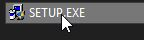
\includegraphics[width=5cm]{figures/5/1174066/0.jpg}
		\centering
		\caption{Setup}
	\end{figure}
	
	\item Setelah itu klik Install
	\begin{figure}[ht!]
		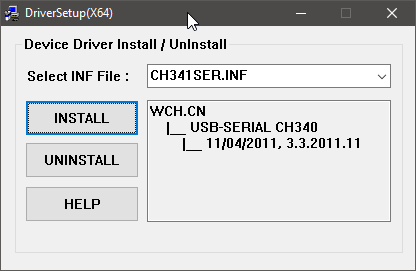
\includegraphics[width=5cm]{figures/5/1174066/1.png}
		\centering
		\caption{Instalasi}
	\end{figure}

	\item Setelah muncul seperti dibawah ini tekan OK
	\begin{figure}[ht!]
		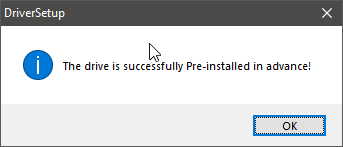
\includegraphics[width=5cm]{figures/5/1174066/2.png}
		\centering
		\caption{Instalasi Berhasil}
	\end{figure}

	\item Hubungkan Arduino ke PC, lalu buka device manager\begin{figure}[ht!]
		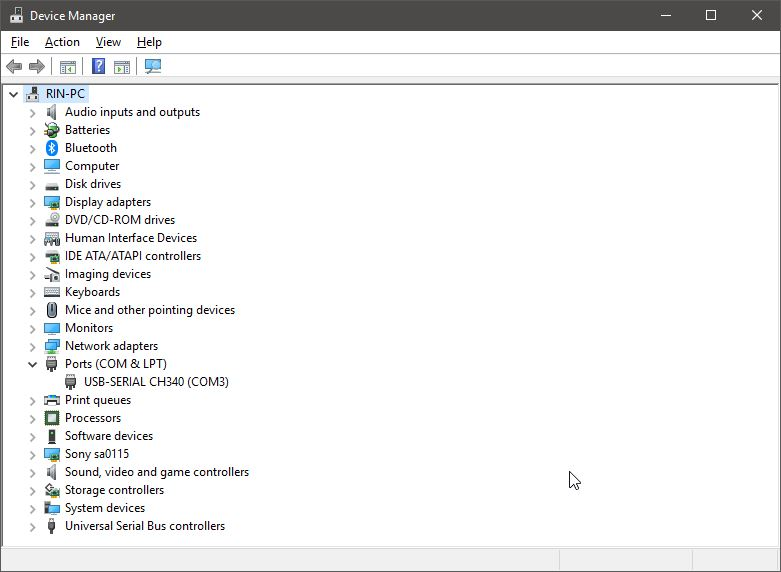
\includegraphics[width=5cm]{figures/5/1174066/3.jpg}
		\centering
		\caption{Device Manager}
	\end{figure}

	\item Lalu pilih pada bagian port apabila seperti ini maka driver arduino telah terinstall\begin{figure}[ht!]
		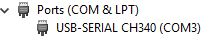
\includegraphics[width=5cm]{figures/5/1174066/4.jpg}
		\centering
		\caption{Arduino Terdeteksi}
	\end{figure}
	
	\end{itemize}

\item Jelaskan bagaimana cara membaca baudrate dan port dari komputer yang sudah terinstall driver

Cara membaca baudrate adalah dengan cara membuka arduino ide lalu mengclik serial monitor yang iconnya seperti kaca pembesar(Cari). 
Untuk mengecek port kita bisa melihatnya melalu device manager pada bagian ports, yang ada tulisan COMXX (XX adalah angka dari COM) itu adalah portnya
	
\item Jelaskan sejarah library pyserial

pySerial adalah modul API Python untuk mengakses port serial. pySerial menyediakan API yang seragam di berbagai sistem operasi, termasuk Windows, Linux, dan BSD.

\item Jelaskan fungsi-fungsi apa saja yang dipakai dari library pyserial

	\begin{itemize}
	\item Serial()
	
	Berfungsi untuk membuka port serial.
	
	\item Write()
	
	Berfungsi untuk mengirimkan data string ke port serial dan mengembalikan nomor bytes yang terkirim.
	
	\item Read(size)
	
	Berfungsi untuk membaca data dari port serial.
	
	\item Readline(size)
	
	Berfungsi untuk membaca line sampai line terakhir (EOL). 
	
	\item Close()
	
	Berfungsi untuk menutup pembacaan port serial.
	\end{itemize}

\item Jelaskan kenapa butuh perulangan dan tidak butuh perulangan dalam membaca serial

Perulangan dalam python berfungsi untuk mengulangi kode/perintah yang ada didalam perulangan tersebut. ada dua macam perulangan pada python, yang pertama for dan yang kedua while.
Perbedaan for dan while adalah for yaitu perulangan yang menghitung (Counted Loop) sedangkan while adalah perulangan yang tidak terhitung (Uncounted Loop). Penggunakan for itu biasanya jika untuk mengulangi kode yang akan ditentukan berapa kali diulangnya sedangkan while digunakan jika ada syarat tertentu untuk mengulangi kode itu dan tidak menentu berapa banyak perulangannya.
Mengapa diperlukan perulangan, karena agar data yang dibaca tidak hanya satu kali saja namun berkali kali, dengan adanya perulangan kita bisa membaca datanya berulang kali. Sehingga data yang kita baca dapat muncul lebih dari satu. Sedangkan kalau kita tidak memakai perulangan maka data yang muncul hanya satu.

\item Jelaskan bagaimana cara membuat fungsi yang mengunakan pyserial

Pembuatan fungsi sama seperti pembuatan fungsi seperti biasanya namun method dari pyserial dimasukkan kedalam fungsi dan dipanggil fungsi yang kita buat tadi
\lstinputlisting[firstline=7, lastline=14]{src/5/1174066/Teori/1174066.py}

\item Scan Plagiarisme
\begin{figure}[ht!]
	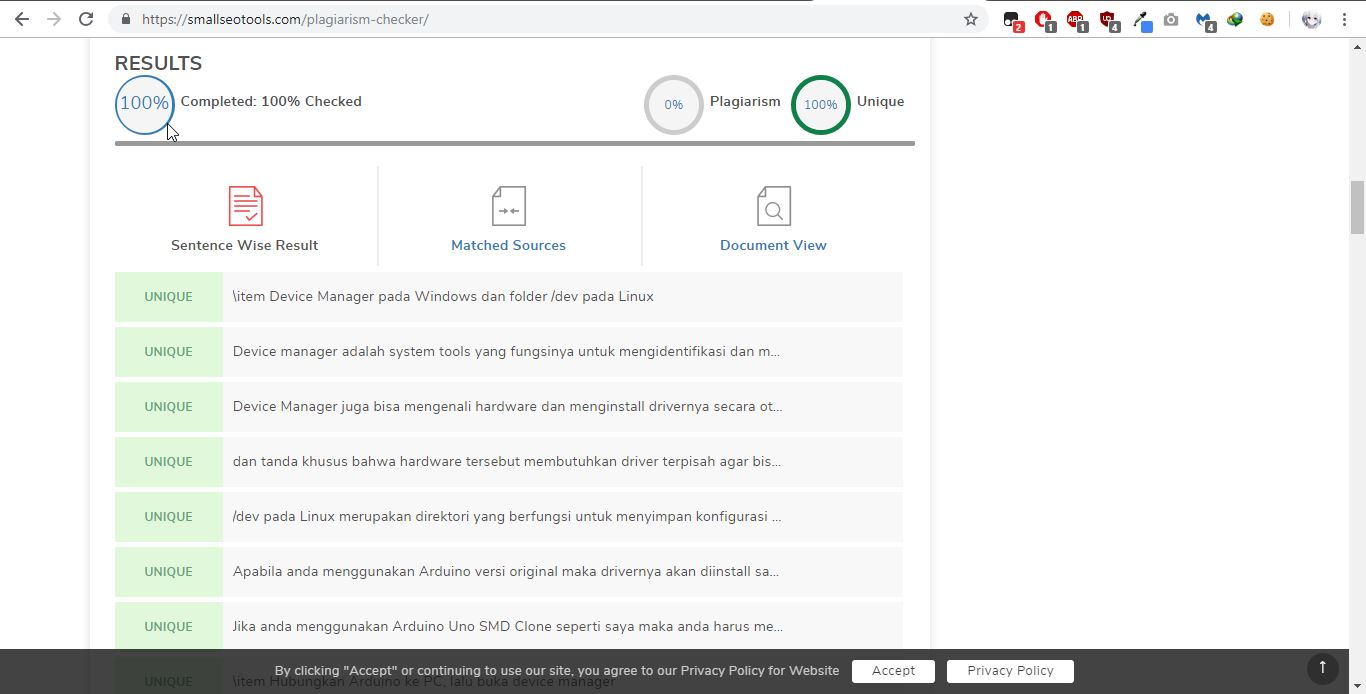
\includegraphics[width=5cm]{figures/5/1174066/plagiat.jpg}
	\centering
	\caption{Plagiarisme}
\end{figure}
\end{enumerate}

%%%%%%%%%%%%%%%%%%%%%%%%%%%%%%%%%%%%%%%%%%%%%%%%%%%%%%%%%%%%%%%%%%%%%%%%%
\section{Difa Al Fansha}
\subsection{Soal Nomor 1}
Apa itu fungsi device manager di windows dan folder /dev di linux?\\
Jawab :
\begin{itemize}
\item Fungsi Device Manager di Sistem Operasi Windows
\end{itemize}
Device manager merupakan program yang mengatur device atau perangkat yang terhuung dengan komputer / laptop.
\begin{itemize}
\item Fungsi Folder /dev di Sistem Operasi Linux
\end{itemize}
Device manager pada linux berada pada folder /dev yang mempunyai arti device. folder ini berisi konfigurasi device pada sistem.

\subsection{Soal Nomor 2}
Jelaskan langkah-langkah instalasi driver dari arduino!\\
Jawab :
\begin{enumerate}
\item Download Software IDE Arduino di https://www.arduino.cc/en/Main/Software
\item Setelah di download jalankan software tersebut.

\item Pilih I Agree.
\begin{figure}[!htbp]
  \centering
  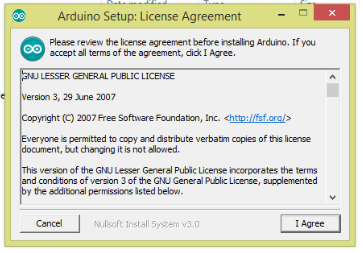
\includegraphics[height=8cm]{figures/5/1174076/Teori/1.PNG}
  \caption{Licence Agreement}
\end{figure}

\item Lalu Next.
\begin{figure}[!htbp]
  \centering
  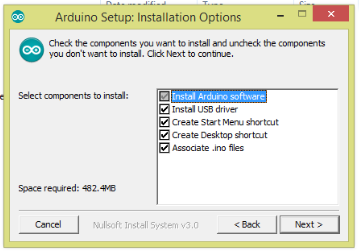
\includegraphics[height=8cm]{figures/5/1174076/Teori/2.PNG}
  \caption{Installation Options}
\end{figure}

\item Pilih directory, lalu tekan Install.
\begin{figure}[!htbp]
  \centering
  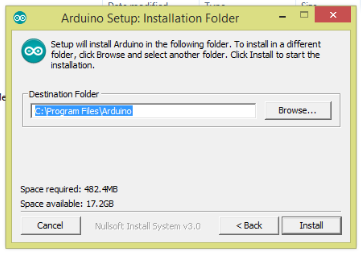
\includegraphics[height=8cm]{figures/5/1174076/Teori/3.PNG}
  \caption{Installation Folder}
\end{figure}

\item Tunggu hingga proses selesai
\begin{figure}[!htbp]
  \centering
  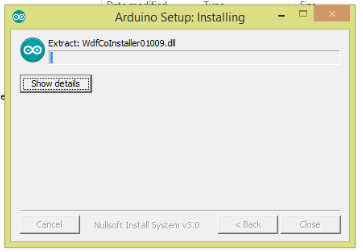
\includegraphics[height=8cm]{figures/5/1174076/Teori/4.PNG}
  \caption{Installation }
\end{figure}

\item Jika sudah selesai, tekan close
\begin{figure}[!htbp]
  \centering
  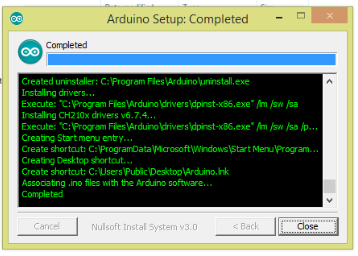
\includegraphics[height=8cm]{figures/5/1174076/Teori/5.PNG}
  \caption{Installing}
\end{figure}
\end{enumerate}

\subsection{Soal Nomor 3}
Jelaskan bagaimana cara membaca baud rate dan port dari komputer yang sudah
terinstall driver! \\
Jawab :\\
baud rate dan port akan langsung terbaca saat arduino dicolokkan ke komputer, sistem akan membaca informasi device yang terhubung.

\subsection{Soal Nomor 4}
Jelaskan sejarah library pyserial!
Jawab : \\
Salah satu cara untuk melakukan komunikasi melalui serial menggunakan python adalah dengan menggunakan modul pyserial. PySerial diluncurkan pada tahun 2002.

\subsection{Soal Nomor 5}
Jelaskan fungsi-fungsi apa saja yang dipakai dari library pyserial!\\
Jawab :\\
\begin{itemize}
\item stop() berguna untuk menghentikan program yang berjalan.
\item readline() berguna untuk membaca sebuah string dari port serial.
\item read(size)berguna untuk membaca jumlah byte dari port serial.
\item close()berguna untuk menutup port serial.
\end{itemize}

\subsection{Soal Nomor 6}
Jelaskan kenapa butuh perulangan dan tidak butuh perulangan dalam membaca serial!\\
Jawab :\\
\begin{itemize}
\item Perulangan
\end{itemize}
Perulangan diperlukan untuk untuk mengulangi perintah agar lebih mudah dan tidak terjadi penumpukan kodingan. Perulangan dijalankan jika kondisi benar dan akan berhenti jika kondisi salah.

\begin{itemize}
\item Tidak membutuhkan perulangan
\end{itemize}
Apabila perintah dijalankan sekali, kita tidak memerlukan perulangan.

\subsection{Soal Nomor 7}
Jelaskan bagaimana cara membuat fungsi yang menggunakan pyserial!\\
Jawab :\\
Definisikan nama fungsi dengan cara def namaFungsi(): lalu masukkan isi fungsi

%%%%%%%%%%%%%%%%%%%%%%%%%%%%%%%%%%%%%%%%%%%%%%%%%%%%%%%%%%%%%%%%%%%%%%%%%%%%%%%%%%%%%%%%%%%%%%%%%%%%%%%%%%%%%%%%%%%%%%%%%%

\section{Fanny Shafira Damayanti | 1174069}
\subsection{Pemahaman Teori}
\begin{enumerate}
\item Fungsi Device manager di Windows dan folder /dev di Linux

Device Manager di Windows berfungsi untuk mengelola semua Hardware yang berada di Windows.

Folder /dev berisikan file device pada Linux.

\item Langkah-langkah Instalasi driver dari arduino

\begin{itemize}
\item Download Software Arduino IDE
\item Hubungkan port USB Arduino ke port pc.
\item setelah itu pc akan mendeteksi driver baru

\begin{figure}[ht!]
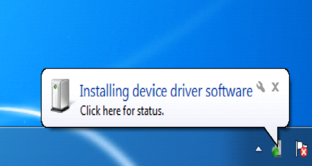
\includegraphics[width=5cm]{figures/5/1174069/1fny.png}
\centering
		\caption{Driver baru}
\end{figure}
	
\item Buka device manager

\begin{figure}[ht!]
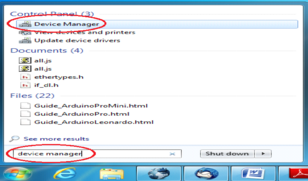
\includegraphics[width=5cm]{figures/5/1174069/2fny.png}
\centering
		\caption{Buka device manager}
\end{figure}
	
	
\item setelah itu, cari "Unknown device"

\begin{figure}[ht!]
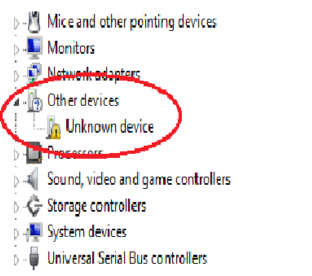
\includegraphics[width=5cm]{figures/5/1174069/3fny.png}
\centering
		\caption{klik "unknown device"}
\end{figure}
	
\item Klik kanan pada "Unknown device" lalu klik Update driver software

\begin{figure}[ht!]
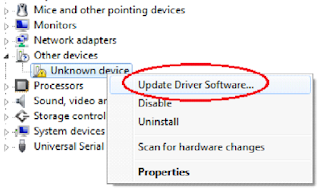
\includegraphics[width=5cm]{figures/5/1174069/4fny.png}
\centering
		\caption{Klik update driver software}
\end{figure}
	
\item Pilih Browse my computer for driver software

\begin{figure}[ht!]
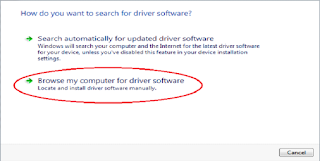
\includegraphics[width=5cm]{figures/5/1174069/5fny.png}
\centering
		\caption{Pilih browse}
\end{figure}
	
\item Cari folder installan Arduino nya

\begin{figure}[ht!]
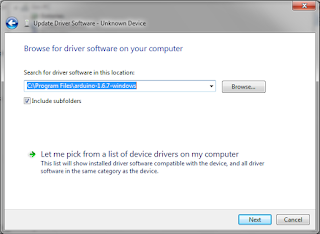
\includegraphics[width=5cm]{figures/5/1174069/6fny.png}
\centering
		\caption{Cari folder instalasinya}
\end{figure}
	
\item Lalu klik next


	
\item setelah itu klik install
\begin{figure}[ht!]
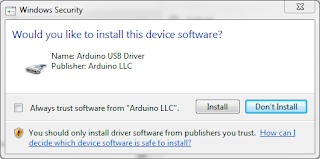
\includegraphics[width=5cm]{figures/5/1174069/7fny.png}
\centering
		\caption{install}
\end{figure}

\item Arduino telah berhasil di install

\begin{figure}[ht!]
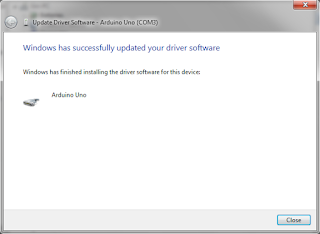
\includegraphics[width=5cm]{figures/5/1174069/8fny.png}
\centering
\caption{selesai}
\end{figure}
	
\end{itemize} 

\item Cara membaca baudrate dan port dari komputer yang sudah terinstall driver

Untuk membaca baudrate dan port yaitu dengan cara :
\begin{itemize}
\item menginstall Arduino IDE
\item setelah itu buka menu serial monitor yang berada di tab tools
\item lalu akan terlihat baudrate dan port yang sedang digunakan.
\end{itemize}

\item Sejarah library pyserial
PySerial merupakan sebuah library yang digunakan untuk komunikasi ke port serial terutama untuk mikrokontroller. PySerial pertama kali diluncurkan pada tahun 2002 yang makin berkembang dalam setiap versinya hingga tahun 2017 lalu.

\item Fungsi-fungsi yang di pakai dari libarary pyserial

\begin{itemize}
			\item \begin{verbatim}stop()\end{verbatim} : untuk menghentikan pembacaan program
			\item \begin{verbatim}serial.to_bytes(sequence)\end{verbatim} : berfungsi untuk mengubah sequence ke dalam bytes agar dapat dikirim ke dalam arduino.
			\item \begin{verbatim}close()\end{verbatim} : untuk menutup port dan menghentikan pembacaan program
		\end{itemize}

\item kenapa butuh perulangan dan tidak butuh perulangan dalam membaca serial

Karena perulangan digunakan untuk membaca seluruh data pada serial yang ada setiap baris. Perulangan digunakan agar data dapat muncul secara terus menerus atau realtime. Sedangkan kalau tidak memakai perulangan, maka data hanya muncul satu kali, tidak berulang.

\item Cara membuat fungsi menggunakan pyserial

\lstinputlisting[firstline=7, lastline=14]{src/5/1174069/Teori/1174069_teori.py}

\item Scan Plagiarisme
\begin{figure}[ht!]
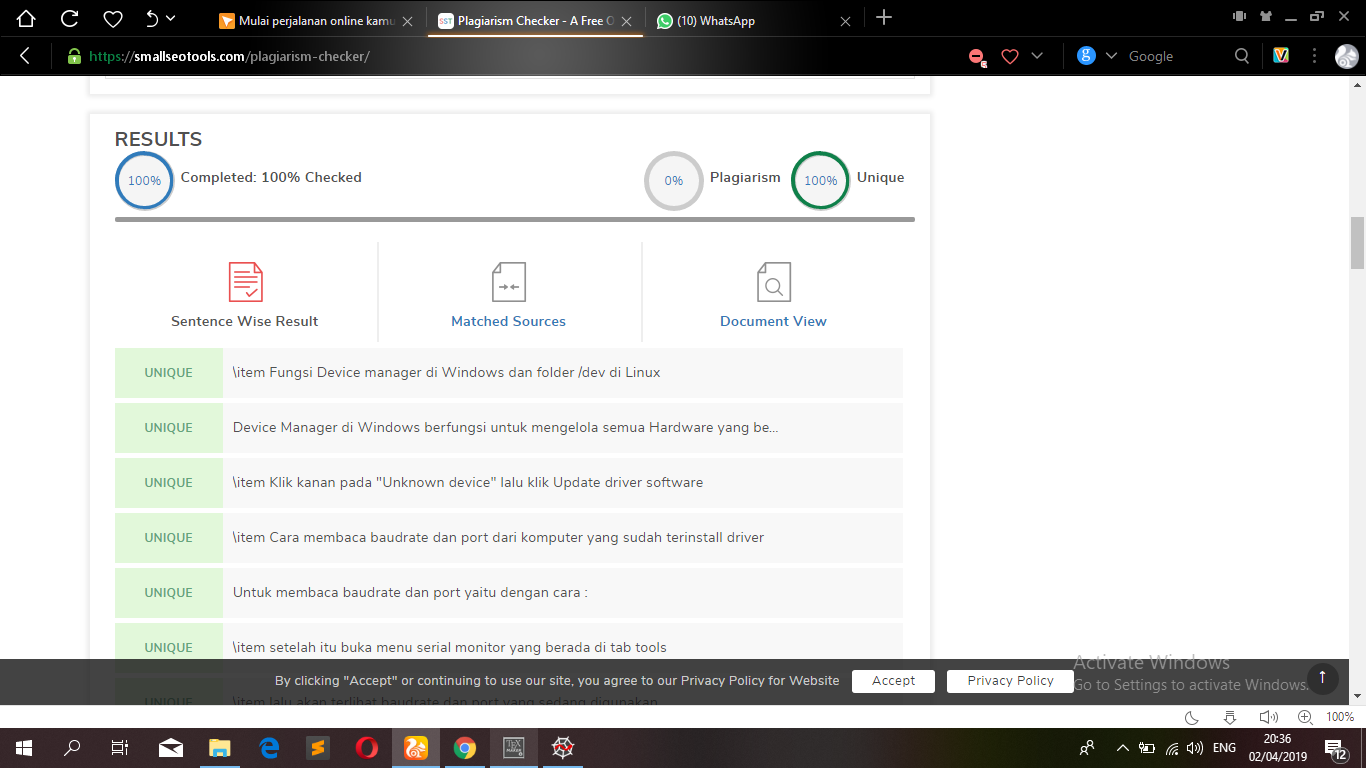
\includegraphics[width=5cm]{figures/5/1174069/plagiarisme.png}
\centering
\caption{plagiarisme}
\end{figure}